\documentclass[11pt]{article}
\usepackage[a4paper,margin=25mm]{geometry}
\usepackage{amsmath,amssymb,booktabs,graphicx,siunitx,enumitem,xcolor,hyperref}
\usepackage{microtype}
\graphicspath{{../figures/corrected_v1/}}
\hypersetup{colorlinks=true,linkcolor=blue,citecolor=blue,urlcolor=blue}
\title{Auditable repeated-service contracts for distribution-connected batteries: separating feeder limits from persistent recovery state}
\author{Siqiang Zhao \and Fengxiang Zhang}
\date{}

\newcommand{\ac}{\mathrm{AC}}
\newcommand{\soc}{\mathrm{SOC}}
\newcommand{\pmax}{P^{\ast}}

\begin{document}
\maketitle

\begin{abstract}
Repeated activation is increasingly used to turn distributed batteries into a flexibility product, yet a single-event operating envelope does not specify what can be delivered after the battery has been only partially re-armed. We formulate an auditable service--recovery contract that composes a persistent state-of-charge (SOC) map with a three-phase AC feeder replay. The contract reports the largest grid-valued export that satisfies terminal-power readback, all non-source phase-voltage limits, line and transformer loading limits, and an SOC reserve for $M$ repeated events. A full-rearm experiment is a pre-registered negative control: when the same measured feeder snapshot and SOC are restored, the admissible set must be invariant. A reserve-limited experiment then carries the SOC deficit between events, making sequence contraction identifiable. We evaluate the frozen contract on 214 training, 71 calibration, and 80 held-out customer-days from the public Ausgrid half-hour data, mapped to an IEEE 13-node OpenDSS snapshot. The selected single-event offer is \SI{140}{kW}; its held-out success rate is 96.25\%. The full-rearm control remains at a median \SI{140}{kW} through six events, whereas the reserve-limited capacity falls to \SI{90}{kW}, \SI{70}{kW}, \SI{50}{kW}, \SI{50}{kW}, and \SI{40}{kW} for two through six events. The negative control and command/readback audit separate a physical recovery-state effect from solver state, telemetry heuristics, or a changing scenario. The resulting workflow is a reproducible interface between flexibility bidding and feeder-level operational validation.
\end{abstract}

\noindent\textbf{Keywords:} battery flexibility; repeated services; recovery contract; distribution feeder; AC power flow; state of charge; operating envelope

\section{Introduction}
Flexibility products are often described by the power that a resource can provide during one activation. For a battery, that description is incomplete: the activation changes the energy state, and a recovery period may be constrained by the same distribution feeder that constrained the service. A product that is feasible once can therefore be infeasible when it is called again. This distinction matters for distribution system operators, aggregators, and market designers because a dispatchable offer must be auditable over the sequence that the offer actually promises.

Several streams of work provide important pieces of this problem. Recovery guarantees for aggregated storage have been formalized in state-space flexibility frameworks \cite{Evans2022Recovery}; security and duration criteria have been developed for distribution resources \cite{Xiao2025SRC}; dynamic feasible operation regions and operating envelopes have been used for coordinated dispatch \cite{Cheng2026FOR,Lankeshwara2025DOE}; and AC-aware flexibility areas have been estimated for charging pools \cite{Giraldo2023RiskEV}. Recovery-constrained flexibility bidding has also been studied in stochastic operation planning \cite{Wanapinit2022FlexBidding}, while communication-dependent planning reserves storage explicitly \cite{Wang2026Communication}. These contributions motivate a careful scope distinction: the object needed here is an operational contract whose repeated service and recovery trajectory is replayed through an unbalanced feeder and whose persistent SOC effect is identified by a negative control.

This paper makes four contributions. First, we define a finite repeated-service contract that composes an SOC transition with a feeder feasibility audit. Second, we introduce an identifiability protocol: identical snapshots with full re-arm must give $C_M=1$, while a non-reset recovery state is the only changing state in the contraction experiment. Third, we implement a state-isolated OpenDSS adapter that measures the realized terminal power of a constant-PQ battery surrogate and reports every non-source phase voltage, line loading, and transformer loading. Fourth, we freeze the offer-selection rule before evaluating chronological held-out customer-days and release all generated tables and figures with the source code.

\section{Contract definition}
\subsection{Service--recovery state map}
Let $s_k$ be the battery SOC immediately before service event $k$, $E$ the usable energy capacity, and $p_k$ positive for feeder export. For a time step $\Delta t$, the SOC update is
\begin{equation}
s_{k+1}=\begin{cases}
s_k-\dfrac{p_k\Delta t}{\eta_d E}, & p_k\ge 0,\\[5pt]
s_k+\dfrac{(-p_k)\Delta t\eta_c}{E}, & p_k<0,
\end{cases}
\label{eq:soc}
\end{equation}
where $\eta_d$ and $\eta_c$ are discharge and charge efficiencies. A service event contains $N_s=4$ half-hour export intervals and $N_r=8$ half-hour recovery intervals. The battery starts at $s_0=0.80$ and must remain above $s_{\min}=0.20$.

For an event-level export command $P$, the full-rearm control uses a recovery power ratio
\begin{equation}
\rho_{\mathrm{rearm}}=\frac{N_s}{N_r\eta_d\eta_c}=0.5540,
\end{equation}
which returns the SOC to its initial value when the AC audit accepts every recovery interval. The persistent-state experiment uses a fixed recovery ratio $\rho_{\mathrm{lim}}=0.30$. Its SOC deficit is passed to the next event. This is a deliberately simple contract state: it exposes whether a repeated offer is backed by a real recovery margin without adding a hidden degradation or temperature model.

\subsection{AC-audited admissible set}
At every service and recovery interval, the command is applied to an isolated OpenDSS context through a single-phase constant-PQ load surrogate. The sign is reversed internally because a positive load consumes power while a positive contract command exports power. The adapter reads the terminal complex power from the circuit element after the nonlinear solve. A command is accepted only if the readback agrees within 1\% (with a \SI{0.01}{kW} absolute floor), the solve converges, all non-source phase voltages lie in [0.95,1.05] pu, and every line and transformer loading ratio is at most 1.0. No zero-voltage phase is silently discarded.

For a profile trajectory $\omega$ and sequence length $M$, the auditable capacity is
\begin{equation}
\pmax_M(\omega)=\max\{P\in\mathcal{G}: \text{AC}(P,\omega,k)=1,\ s_{k,j}\ge s_{\min}\ \forall k\le M\},
\label{eq:capacity}
\end{equation}
where $\mathcal{G}=\{0,10,\ldots,300\}$ kW and $j$ indexes the service and recovery intervals. We report the contraction ratio $C_M=\pmax_M/\pmax_1$. Under an unchanged deterministic snapshot and full re-arm, Eq.~\eqref{eq:capacity} is invariant by construction. This is a required negative control rather than a result that is assumed after the fact.

\section{Data and experimental design}
\subsection{Interval-resolved profiles}
The main evaluation uses the public Ausgrid solar-home data \cite{Ausgrid2011}. GC and CL channels are combined as load and GG is used as PV. The source values are energy per half-hour and are converted to average kW by dividing by 0.5 h. Ten customer groups are created once with a fixed seed; each group retains a 48-point day trajectory. Dates are split chronologically within each month before any outcome is calculated: 214 training days, 71 calibration days, and 80 test days. A separate loader also corrects the cumulative-energy convention in the OPSD household release \cite{OPSD2020}; those profiles are retained as an external data audit rather than mixed into the main offer selection.

The measured profiles are mapped to the feeder through a fixed stress embedding. Train-only maxima define $l_{\mathrm{norm}}$ and $g_{\mathrm{norm}}$; the factors used in every split are
\begin{equation}
l=\operatorname{clip}(0.40+0.30l_{\mathrm{norm}},0.35,0.85),\qquad
g=\operatorname{clip}(0.10+0.60g_{\mathrm{norm}},0,1).
\end{equation}
The mapping makes the profile shape and chronological split auditable without claiming that a household load is numerically equal to the IEEE feeder load.

\subsection{Feeder and offer selection}
The network is the public IEEE 13-node snapshot \cite{OpenDSS13}. A battery is placed at the valid phase-specific site 611.3 and a 300 kW fixed-P PV surrogate at 675.1. The OpenDSS context is rebuilt before every candidate event so that a failed high-power solve cannot contaminate a later candidate. Candidate offers are evaluated over the two fixed daily service starts (intervals 8 and 32). The largest grid offer with at least 95\% successful events on the training dates is selected. Calibration dates choose the largest predeclared multiplier from {0.80, 0.90, 1.00} that retains the 95\% threshold. Test dates are then read with all parameters frozen.

\section{Results}
\subsection{Offer selection and held-out audit}
The frozen offer is \SI{140}{kW}. The success rates are 98.13\% on training events, 97.18\% on calibration events, and 96.25\% on the 160 held-out events (80 dates and two starts per date). The maximum held-out phase voltage is 1.0506 pu; the few failed events are retained in the audit rather than removed. The corresponding voltage and success scatter is shown in Fig.~\ref{fig:audit}. A direct command/readback test at -70, 0, 70, and \SI{140}{kW} gives terminal powers within \SI{0.005}{kW} of the command (Fig.~\ref{fig:readback}).

\begin{figure}[t]
\centering
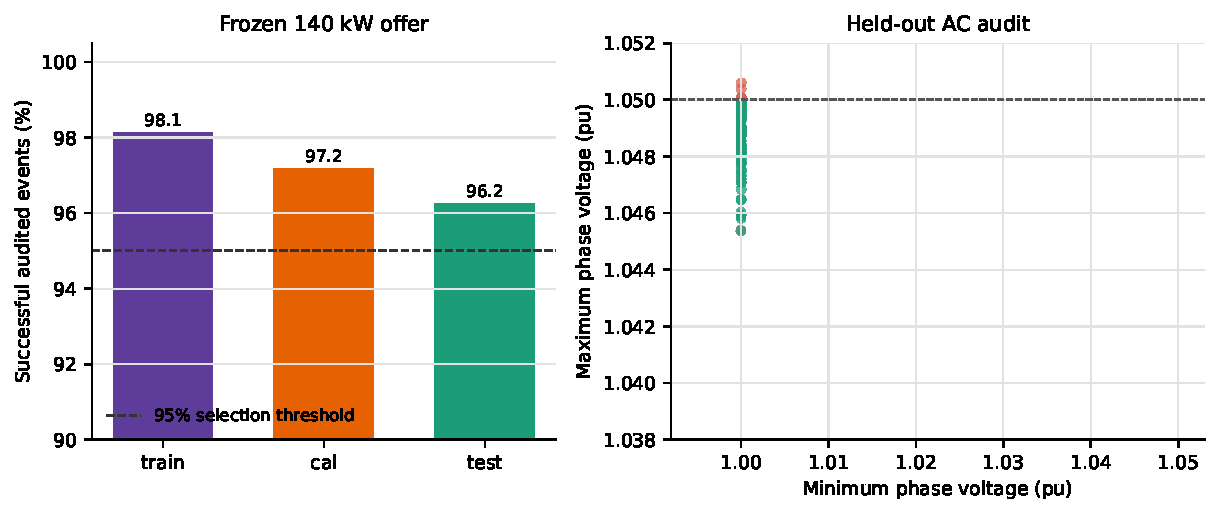
\includegraphics[width=0.98\linewidth]{fig3_heldout_ac_audit}
\caption{Frozen-offer success rates and held-out voltage audit. The dashed line in the left panel is the predeclared 95\% threshold; the right panel retains both accepted and rejected test events.}
\label{fig:audit}
\end{figure}

\subsection{Sequence contraction and negative control}
The full-rearm control repeats an identical held-out profile and restores the SOC after each event. Its two-event contraction ratio is $C_2=1.0$. Across the 80 test days, the full-rearm capacity has a median of \SI{140}{kW} for every $M=1,\ldots,6$ (test-day range 130--140 kW). In contrast, the reserve-limited capacity has medians of \SI{140}{kW}, \SI{90}{kW}, \SI{70}{kW}, \SI{50}{kW}, \SI{50}{kW}, and \SI{40}{kW} for $M=1$ through 6, respectively. Thus $C_2=0.643$ and $C_6=0.286$ relative to the reserve-limited single-event capacity. The state trajectory in Fig.~\ref{fig:soc} shows why the contraction is identifiable: the full-rearm state returns to 0.80, whereas the limited recovery leaves a persistent deficit that reaches the reserve boundary.

\begin{figure}[t]
\centering
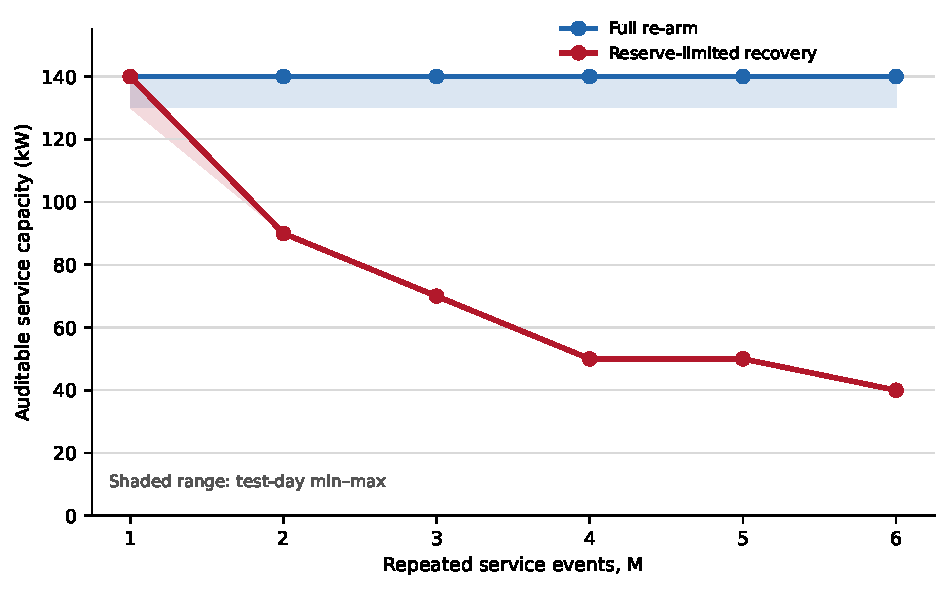
\includegraphics[width=0.73\linewidth]{fig2_sequence_capacity}
\caption{Sequence capacity on held-out profiles. The blue curve is the full-rearm negative control; the red curve carries the reserve-limited SOC state. Shading shows the test-day minimum and maximum.}
\label{fig:sequence}
\end{figure}

\begin{figure}[t]
\centering
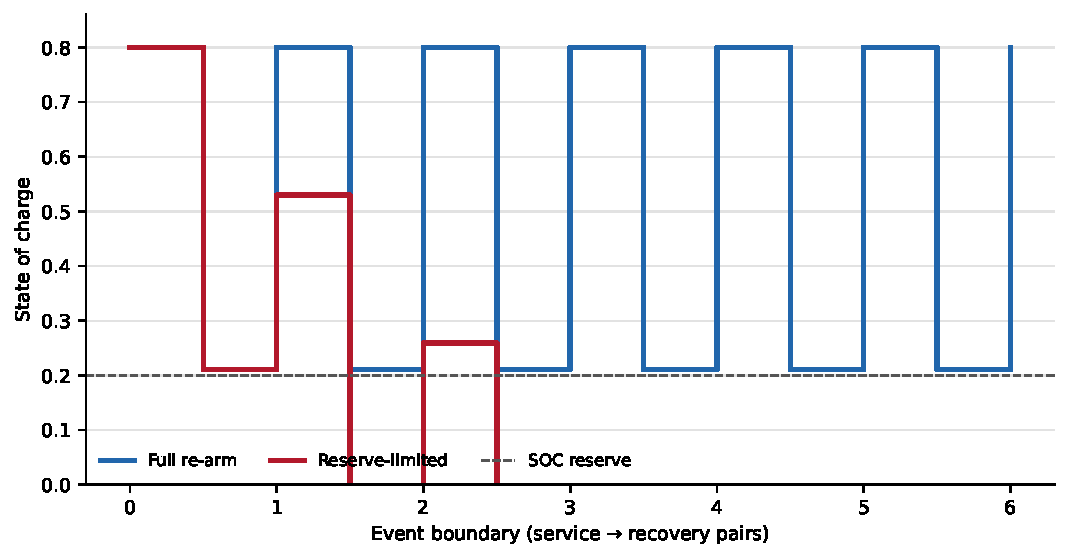
\includegraphics[width=0.82\linewidth]{fig4_soc_state_trace}
\caption{SOC state for a \SI{140}{kW} repeated event. Full re-arm returns to the initial state after each recovery; the reserve-limited contract carries the deficit forward.}
\label{fig:soc}
\end{figure}

\begin{figure}[t]
\centering
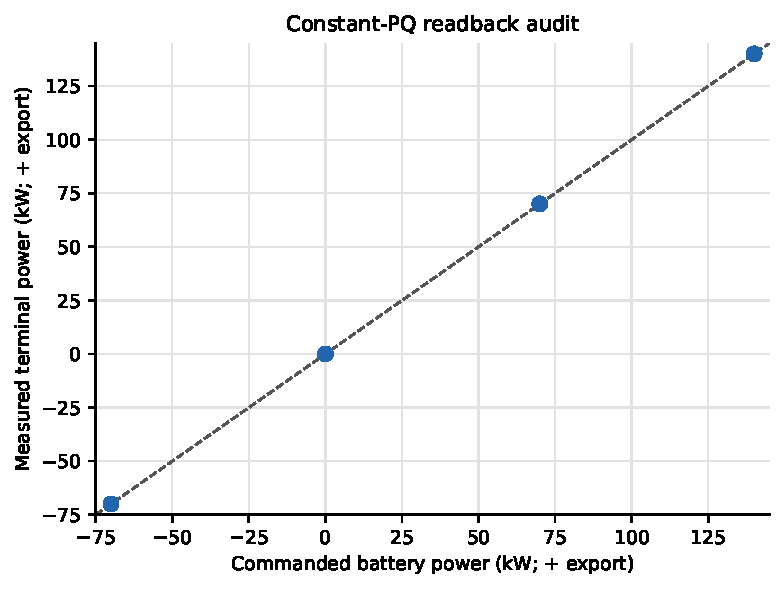
\includegraphics[width=0.76\linewidth]{fig6_command_readback}
\caption{Measured terminal power versus commanded battery power at the held-out operating point. Positive values export to the feeder.}
\label{fig:readback}
\end{figure}

\section{Discussion}
The results answer a narrow operational question. A one-event offer can be valid on more than 96\% of unseen profile events, yet that statistic alone does not describe repeated delivery. When the recovery contract restores the state, the repeated capacity is invariant up to the 10 kW grid and the small AC variation across test days. When recovery is intentionally limited and the state is carried forward, the sequence capacity contracts predictably. The negative control prevents attributing the contraction to an unobserved change in the feeder scenario.

The contribution is complementary to dynamic operating envelopes, risk-aware AC flexibility areas, recovery-aware bidding, and duration assessment. Those methods can supply a richer uncertainty model or a market objective; the interface developed here supplies a sequence-level acceptance test that can be applied after such a model proposes an offer. Communication or telemetry effects are deliberately excluded from the headline result because a deterministic derating formula would confound information value with a preselected penalty.

There are three limits. The IEEE 13-node feeder is a public validation network rather than a utility feeder, and the profile-to-feeder mapping is a declared stress embedding. The battery state contains SOC but no temperature, degradation, or converter fault state. Finally, the 10 kW grid and fixed recovery ratio quantify one contract design; they do not establish a universal tariff. These limits define straightforward extensions: multi-phase inverter models, stochastic measurement uncertainty, learned recovery policies, and field feeder telemetry can all be inserted without changing the identifiability protocol.

\section{Conclusions}
We developed and audited a repeated-service contract that joins persistent SOC recovery with three-phase feeder feasibility. The physically isolated adapter, chronological public-profile split, and full-rearm negative control make the sequence effect testable. In the corrected experiment, a frozen \SI{140}{kW} offer achieved 96.25\% held-out event success; its capacity stayed at \SI{140}{kW} under full re-arm but fell to \SI{40}{kW} by the sixth reserve-limited event. The result supports a practical rule for flexibility products: the offered power should be accompanied by an explicit recovery state and an auditable sequence horizon.

\section*{CRediT authorship contribution statement}
Siqiang Zhao: Conceptualization, Methodology, Software, Validation, Formal analysis, Investigation, Data curation, Visualization, Writing -- original draft. Fengxiang Zhang: Supervision, Writing -- review and editing.

\section*{Declaration of competing interest}
The authors declare that they have no known competing financial interests or personal relationships that could have appeared to influence the work reported in this paper.

\section*{Funding}
No dedicated external funding was received for this work.

\section*{Declaration of generative AI and AI-assisted technologies in the writing process}
During preparation of this manuscript, the authors used OpenAI Codex/ChatGPT and Manus to assist with code organization, literature checking, and language editing. The authors reviewed and verified all content, analyses, and conclusions and remain fully responsible for the work.

\section*{Data and code availability}
The corrected scripts, manifests, figures, and tests are supplied with the submission package. The code is released under the MIT License at \url{https://github.com/Zhaosiqiang/RecoveryFlex-AE}. A persistent DOI archive can be added after editorial review without changing the release commit.

\bibliographystyle{unsrt}
\bibliography{references}
\end{document}
